\documentclass[border=10pt]{standalone}
\usepackage{tikz}
\usetikzlibrary{arrows.meta,calc}

\begin{document}
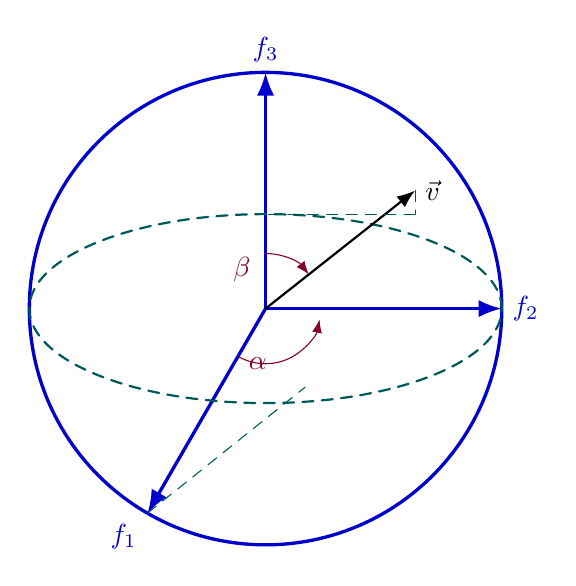
\begin{tikzpicture}[>=Latex,line join=round,line cap=round,
  bluevec/.style={blue!80!black,very thick},
  proj/.style={dash pattern=on 4pt off 3pt,thick,teal!70!black},
  projthin/.style={dash pattern=on 4pt off 3pt,thin,teal!70!black},
  angle/.style={purple!70!black,->,thin}]
  
  % Parameters
  \def\R{3}                % radius of outer circle
  \def\ael{3}              % ellipse x radius
  \def\bel{1.2}            % ellipse y radius
  
  % Basic axes directions
  \coordinate (O) at (0,0);
  \coordinate (F2) at (\R,0);
  \coordinate (F3) at (0,\R);
  % f1 roughly at -120 degrees on circle
  \coordinate (F1) at ({\R*cos(240)},{\R*sin(240)});
  
  % Vector v
  \coordinate (V)  at (1.9,1.5);
  % Projection of v onto ellipse horizontally
  \coordinate (VprojE) at (1.9,\bel);     % vertical drop to ellipse plane
  \coordinate (VprojZ) at (0,\bel);       % horizontal to vertical axis
  
  % Point on ellipse from f1 projection
  \coordinate (F1proj) at (0.5,-1.0);
  
  % Outer circle
  \draw[bluevec] (O) circle (\R);
  
  % Basis vectors
  \draw[bluevec,->] (O) -- (F3) node[above,blue!80!black] {$f_3$};
  \draw[bluevec,->] (O) -- (F2) node[right,blue!80!black] {$f_2$};
  \draw[bluevec,->] (O) -- (F1) node[below left,blue!80!black] {$f_1$};
  
  % Ellipse (equatorial)
  \draw[proj] (0,0) ellipse ({\ael} and {\bel});
  
  % Dashed projection from f1 tip to ellipse
  \draw[projthin] (F1) -- (F1proj);
  
  % Vector v
  \draw[->,thick] (O) -- (V) node[right] {$\vec v$};
  
  % Projections of v
  \draw[projthin] (V) -- (VprojE);
  \draw[projthin] (VprojE) -- (VprojZ);
  
  % Angle alpha between f1 and horizontal projection of v
  % Define direction of horizontal projection ray
  \coordinate (Ralpha) at (1,-0.2); % some direction into 4th quadrant / first
  \draw[angle] (O) ++({atan2(-2.598,-1.5)}:0.7) 
               arc[start angle={atan2(-2.598,-1.5)},
                   end angle={atan2( -0.2,1)},
                   radius=0.7];
  \node[purple!70!black] at (-0.1,-0.7) {$\alpha$};
  
  % Angle beta between vertical axis and v
  \draw[angle] (O) ++(90:0.7)
               arc[start angle=90,
                   end angle={atan2(1.5,1.9)},
                   radius=0.7];
  \node[purple!70!black] at (-0.3,0.5) {$\beta$};
  
\end{tikzpicture}
\end{document}